\documentclass[11pt]{article}

\usepackage[a4paper,margin=24mm]{geometry}
\usepackage{amsmath,amssymb,amsthm,mathtools}
\usepackage{booktabs,tabularx,array}
\usepackage{graphicx}
\usepackage{flafter}
\usepackage{xcolor}
\usepackage{enumitem}
\usepackage[hidelinks]{hyperref}

\newtheorem{theorem}{Theorem}[section]
\newtheorem{proposition}[theorem]{Proposition}
\newtheorem{corollary}[theorem]{Corollary}
\newtheorem{lemma}[theorem]{Lemma}
\theoremstyle{definition}
\newtheorem{assumption}[theorem]{Assumption}
\newtheorem{definition}[theorem]{Definition}
\theoremstyle{remark}
\newtheorem{remark}[theorem]{Remark}

\newcommand{\C}{\mathbb C}
\newcommand{\R}{\mathbb R}
\newcommand{\Aset}{\mathcal A}
\newcommand{\Yset}{\mathcal Y}
\newcommand{\Disc}{\mathbb D}
\newcommand{\Kest}{\mathcal K_{\rm est}}
\newcommand{\Mtar}{\mathcal M}
\newcommand{\diameter}{\operatorname{diam}}
\newcommand{\status}[1]{\texttt{#1}}

\title{Certified Identifiability of Fractional ECG Harmonic Surrogates\\
from Multi-Rate Records}
\author{Anonymous authors}
\date{}

\begin{document}
\maketitle

\begin{abstract}
We study when a scalar fractional harmonic surrogate can be identified from
surface-ECG windows acquired at different heart rates.  The object of
inference is an effective input--output order, not an internal cardiac state
or a physiological fractional mechanism.  For the asymptotic harmonic branch
of a dimensionless Caputo model with unknown common complex morphology and
positive real damping, we prove
that one exact complex rate response is insufficient and two are globally
sufficient.  The proof constructs a complete common-gain quotient whose
physical image is explicit and whose inverse is unique on
$(0,1]\times\R_{>0}$.  We extend the result to an exact multi-rate consistency
test, and prove two limits: unrestricted rate-specific complex morphology
destroys order identifiability, while any positive independent morphology
disk prevents singleton recovery locally in the two-rate known-damping
problem.  For finite records, we connect fixed-phase complex weighted least
squares, independently calibrated residual bounds, joint response-disk set
inversion, validated Gram margins, and a fail-closed replay certificate.
Specializing the standard reliable-set minimax principle to the gauge-reduced
response disks gives an exact separation threshold for rate-window design.
Deterministic sweeps recovered all 1,260 exact two-rate cases, preserved all
common-gain invariants, and detected all 1,260 independently valid but
three-rate-inconsistent controls.  A
design-locked four-record Fantasia engineering pilot replayed 1,859/1,859 WLS
records, but all four fractional fits terminated at $\alpha=1$ and none
materially improved on the nested $\alpha=1$ model.  The distinct
fractional-order hypothesis is therefore \status{NOT\_SUPPORTED}; because
several acquisition and model-error primitives remain uncalibrated, all four
real records are also \status{NOT\_CERTIFIABLE}.  The negative result is part
of the proposed certification discipline rather than evidence for a cardiac
digital twin.
\end{abstract}

\noindent\textbf{Keywords:} fractional-order systems; structural
identifiability; set-membership estimation; electrocardiography; validated
numerics; experiment design.

\section{Introduction}

Fractional differential models provide compact representations of memory and
power-law relaxation.  They have been used in ECG signal generators and
cardiac rhythm models \cite{das2013,templos2021,takha2024}, while Kalman-type
filters for fractional systems already estimate states, parameters, and order
\cite{sierociuk2006,sierociuk2021,yu2026}.  These precedents make it
scientifically inappropriate to present either a fractional ECG model or a
fractional extended Kalman filter as the contribution by itself.  The harder
control question is prior to filtering: under which phase, morphology,
damping, and uncertainty contracts is the effective order identifiable from
a finite collection of ECG rate windows?

The distinction matters because a surface ECG is a low-dimensional projection
of a distributed electrophysiological process.  Even detailed cardiac-twin
inverse problems can have severe nonuniqueness
\cite{gillette2021,grandits2025}.  A flexible rate-specific gain can likewise
make a simple harmonic surrogate fit every candidate order.  A point estimate
returned by an optimizer therefore does not establish either identifiability
or physiological meaning.  A defensible workflow must expose the nuisance
gauge, give a finite-record coverage statement, and refuse a conclusion when
the required error bounds are absent.

This paper develops such a workflow for the declared scalar harmonic model.
Its contributions are deliberately narrow.

\begin{enumerate}[leftmargin=*,itemsep=2pt]
\item We construct a complete common-complex-gain quotient and prove global
      two-rate recovery of order and damping.  One rate is strictly
      insufficient, and a third rate supplies a redundant exact
      consistency equation.
\item We characterize the boundary of the claim: rate-specific complex
      morphology eliminates order information; positive independent
      morphology disks preclude local point recovery; and finite frequency
      responses cannot distinguish a fractional mechanism from a stable
      rational interpolant.
\item We formulate the finite-data problem as a joint response-disk inversion.
      A conditional data-to-disk theorem separates WLS geometry from
      independently calibrated history, dwell, phase, sampling, front-end,
      noise, and model-discrepancy budgets.  Validated Gram and replay checks
      fail closed rather than silently shrinking uncertainty.
\item We specialize the standard reliable-set minimax identity and exact
      product-disk separation threshold to the common-gauge ECG geometry and
      its certified R2 radii, turning heart-rate/window selection into an
      operational worst-case set-diameter design problem.
\item We report both positive synthetic checks and a negative four-record
      Fantasia pilot.  The latter supports the reproducibility of the signal
      processing path, but not a distinct fractional order and not a certified
      real-ECG response disk.
\end{enumerate}

Detailed proofs, validated-continuation constructions, and all component
bounds are given in the accompanying theory-core supplement.  The present
paper retains only the results needed to understand the control contribution
and its empirical boundary.

For cross-document navigation, the supplement numbers the quotient geometry,
global two-rate inverse, and reference-pair consistency as S4, S5, and S7;
the forward-disk and morphology-drift results as S13 and S15; the analytic
selector tube and conditional WLS enclosure as S32 and S39; the exact-payload
enclosure and R2 component/transfer results as S44, S46, and S47; and the
reliable-set/design results as S52 and S54.

\section{Related work and claim boundary}

\subsection{Fractional identification and set membership}

Frequency-domain identifiability of fractional systems and its sensitivity
limits are established topics \cite{nazarian2010}.  Malti et al. studied
set-membership estimation for an isomorphic first-order fractional transfer
model using bounded complex frequency data \cite{malti2010}; Khemane et al.
developed robust frequency-domain estimation under rectangular, polar, and
disk uncertainty descriptions \cite{khemane2012}.  Robust fractional
experiment design and general nonlinear set-membership design also predate
this work \cite{abrashov2017,karimshoushtari2020}.  Consequently, neither
complex disks, interval inversion, nor experiment design is claimed as a
generic novelty here.

The specialization pursued below is the interaction among (i) a common
unknown complex ECG morphology/lead gauge, (ii) positive real damping, (iii)
multi-rate phase-locked harmonic responses, and (iv) a finite-record
certificate whose evidence objects can be replayed.  Validated linear algebra
and parameter-dependent enclosures follow standard principles
\cite{neumaier1989,rump2010,goldsztejn2006,ponleitner2021}; our contribution is
the model geometry and the composition semantics, not a new interval-Newton
method.

\subsection{Fractional ECG and Kalman models}

The integer-order McSharry generator \cite{mcsharry2003} and its nonlinear
Bayesian filtering descendants \cite{sameni2007} established dynamical ECG
state-space modelling well before the present study.  Fractional ECG
generators and McSharry extensions have also been reported
\cite{das2013,takha2024}.  Fractional Kalman filters have a substantial
history \cite{sierociuk2006,sierociuk2021,yu2026}.  We therefore do not claim
a new ECG generator, a generic fractional filter, observer stability under
fractional-order mismatch, or direct recovery of cardiac tissue states.

Our model is a \emph{surface-ECG harmonic surrogate}.  Its order is an
effective parameter inside a declared family.  The present evidence does not
meet the subject-specific synchronization and held-out predictive standard
needed to call the construction a cardiac digital twin.

\section{Problem formulation}

\subsection{Dimensionless harmonic surrogate}

Fix a reference time $\tau_\star>0$, set $\xi=t/\tau_\star$, and consider
\begin{equation}
 {}^C D_\xi^\alpha z(\xi)
 =-\lambda z(\xi)+\sum_{m\in\mathbb Z}q_m e^{im\theta(\xi)} .
 \label{eq:time-model-main}
\end{equation}
Here $\lambda$ is dimensionless and $q_m$ has the measurement unit of $z$.
We do not interpret \eqref{eq:time-model-main} with a finite lower terminal as
possessing an exact periodic orbit: time-invariant Caputo systems generally do
not \cite{tavazoei2009}.  The response below is the infinite-history (Weyl)
harmonic branch, equivalently the asymptotic periodic component of the
finite-terminal Caputo solution \cite{duan2022}.  Initial-condition,
prehistory, and finite-dwell transients are separate terms in the
data-to-response-disk coverage gate (R2).  At
one positive harmonic and rate $r$, this branch is
\begin{equation}
 Z_r=\frac{q}{\lambda+(i\nu_r)^\alpha},\qquad
 (i\nu)^\alpha=\nu^\alpha e^{i\pi\alpha/2},
 \label{eq:response-main}
\end{equation}
with
\[
 \alpha\in I=[\alpha_-,1],\quad 0<\alpha_-<1,
 \qquad \lambda\in\Lambda\Subset\R_{>0},\qquad q\in\C\setminus\{0\}.
\]
The dimensionless frequency is $\nu_{r,m}=m\tau_\star\Omega_r$, where
$\Omega_r$ is the base angular heart rate in rad/s.  A common nonzero complex
lead gain is absorbed into $q$.  For real ECG, the negative harmonic
is the conjugate of the positive one and does not add an independent model
equation.

\begin{assumption}[Declared information boundary]
\label{ass:boundary-main}
Rates are known, positive, and distinct.  Responses share one R-peak phase
anchor, one causal preprocessing chain, the principal fractional branch, and
common $(\alpha,\lambda,q)$.  No uncalibrated rate-specific complex gain,
phase, or delay is allowed.  Any restitution or acquisition bound used in a
certificate is calibrated independently of the identification residual.
\end{assumption}

The estimator may use a two-sided basis $\Kest\subset\mathbb Z$, including DC
and conjugate negative harmonics.  The identification targets
$\Mtar\subset\mathbb N_{>0}$ contain only positive harmonics.  This distinction
prevents DC or a duplicated conjugate coefficient from entering formulae that
use $\log\nu$.

\subsection{Finite-window estimator and response disks}

In a digital window with exact integer endpoints $j_a<j_b$ spanning $N$
complete detected RR intervals, let $j_n\in[j_a,j_b)$ be the selected sample
indices, $w_n>0$, and $\sum_n w_n=1$.  Freeze the whole-window phase
\[
 \widehat\phi_n=2\pi N\frac{j_n-j_a}{j_b-j_a},\qquad
 \Psi_{n,k}=e^{ik\widehat\phi_n},\quad k\in\Kest .
\]
The implementation never reconstructs this phase through rounded binary64
seconds; timestamp uncertainty is budgeted separately.
With $W=\operatorname{diag}(w_n)$ and $G=\Psi^*W\Psi$, the joint complex WLS
coefficient and front-end-corrected target are
\begin{equation}
 \widetilde{\boldsymbol C}=G^{-1}\Psi^*W\boldsymbol y,\qquad
 \widetilde Z_m=\widetilde C_m/\widehat H_m .
 \label{eq:wls-main}
\end{equation}
The real-signal convention is
$y=Z_0+2\operatorname{Re}\sum_{m>0}Z_m e^{im\phi}$; a one-sided sinusoidal
amplitude is not substituted for the complex Fourier coefficient.
In finite-window formulae, $\widehat H_m$ abbreviates the calibrated
$\widehat H_{r,m}$ for the current rate/window.  Values may vary with physical
frequency under the one frozen causal front end; no uncalibrated rate-specific
gain is absorbed into the morphology.

The inference layer receives disks
\begin{equation}
 |Z_{r,m}-\widetilde Z_{r,m}|\le\epsilon_{r,m}.
 \label{eq:disk-main}
\end{equation}
The centre and radius have different evidentiary roles: the centre is replayed
from the named window payload, whereas every contribution to the radius needs
an independent deterministic or simultaneous probabilistic contract.

\subsection{Decision semantics}

We distinguish four protocol-level outcomes:
\[
 \status{PASS\_DETERMINISTIC},\quad
 \status{PASS\_PROBABILISTIC},\quad
 \status{NOT\_CERTIFIABLE},\quad
 \status{EXCLUDE\_PROTOCOL}.
\]
\status{PASS\_PROBABILISTIC} requires a predeclared simultaneous-coverage
contract and an explicit joint failure-probability bound.
\status{EXCLUDE\_PROTOCOL} means that the acquisition or preprocessing design
violates the information boundary---for example, a noncausal target-window
operation or an uncalibrated rate-specific amplitude/phase normalization---so
the protocol is ineligible for inference.  Missing bounds, singular Gram
geometry, a wide nonempty order set, or a broken hash chain instead produce
\status{NOT\_CERTIFIABLE}; none is evidence that the model is false.  The
separate downstream relation \status{REJECT\_MODEL} requires a complete joint
outer proof of emptiness with no unresolved branch; it is not an R2 protocol
status.

The empirical label \status{NOT\_SUPPORTED}, used only in the held-out model
comparison below, is not a fifth certificate relation.  It means that the
predeclared material-improvement threshold was not met.  It is neither
\status{NOT\_CERTIFIABLE} nor model rejection, does not prove that
$\alpha<1$ or the full model family is false, and may coexist with
\status{NOT\_CERTIFIABLE}.

\section{Structural identifiability and its limits}

\subsection{A complete common-gain quotient}

For two nonzero responses let $W_r=Z_r^{-1}$,
$D=W_2-W_1$, and $C=W_1/D$ when $D\ne0$.  The number $C$ is invariant under
$(Z_1,Z_2)\mapsto(gZ_1,gZ_2)$ for any $g\in\C\setminus\{0\}$.  It is also
complete: equality of $C$ for two ordered pairs implies that the pairs differ
by one common nonzero complex gain.

\begin{proposition}[One rate is insufficient]
For one exact response $Z_1$, the order is not structurally identifiable.
\end{proposition}
\begin{proof}
For every candidate $(\beta,\ell)\in I\times\Lambda$, the nonzero choice
$q_{\beta,\ell}=Z_1[\ell+(i\nu_1)^\beta]$ reproduces $Z_1$.
\end{proof}

\begin{theorem}[Global two-rate recovery modulo a common complex gauge]
\label{thm:two-rate-main}
Let $0<\nu_1<\nu_2$ and suppose two exact responses satisfy
\eqref{eq:response-main}.  Put $\varrho=\nu_2/\nu_1>1$.  Then $D\ne0$,
$\operatorname{Im}C<0$, and the true order is the unique
$\beta\in(0,1]$ satisfying
\begin{equation}
 (\varrho^\beta-1)
 \left[\operatorname{Re}C+
 \operatorname{Im}C\cot\left(\frac{\pi\beta}{2}\right)\right]=1.
 \label{eq:root-main}
\end{equation}
After recovering $\alpha$,
\begin{equation}
 q=\frac{e^{i\pi\alpha/2}(\nu_2^\alpha-\nu_1^\alpha)}{D},
 \qquad
 \lambda=\nu_1^\alpha e^{i\pi\alpha/2}
 [C(\varrho^\alpha-1)-1]\in\R_{>0}.
 \label{eq:recovery-main}
\end{equation}
Equivalently, the quotient map
\begin{equation}
 \Phi_{\varrho}(\alpha,\kappa)=
 \frac{1+\kappa e^{-i\pi\alpha/2}}{\varrho^\alpha-1},
 \qquad \kappa=\lambda/\nu_1^\alpha,
 \label{eq:quotient-map-main}
\end{equation}
is one-to-one from $(0,1]\times\R_{>0}$ onto
\[
 \mathcal Q_\varrho=
 \{u+iv:u\ge(\varrho-1)^{-1},\ v<0\}.
\]
It is a diffeomorphism between the corresponding interiors.
\end{theorem}

\begin{proof}[Proof idea]
Inverse-response subtraction eliminates damping and gives
$D=e^{i\pi\alpha/2}(\nu_2^\alpha-\nu_1^\alpha)/q$.  Hence
\[
 C=\frac{1+\kappa e^{-i\pi\alpha/2}}{\varrho^\alpha-1},
 \qquad \kappa>0.
\]
For a candidate $\beta$, requiring the reconstructed damping to be real is
exactly \eqref{eq:root-main}.  Substitution of the true quotient reduces the
candidate equation to
\[
 \varrho^\beta-\varrho^\alpha
 +\kappa(\varrho^\beta-1)
 \frac{\sin[\pi(\beta-\alpha)/2]}{\sin(\pi\beta/2)}=0.
\]
Both terms have the sign of $\beta-\alpha$, proving uniqueness.  Positivity
of the reconstructed damping follows from $\operatorname{Im}C<0$.  Surjectivity
onto $\mathcal Q_\varrho$ follows by the same sign argument at the interval
endpoints.  Finally,
\[
 \det\frac{\partial(\operatorname{Re}C,\operatorname{Im}C)}
 {\partial(\alpha,\kappa)}=
 \frac{\varrho^\alpha\log\varrho\sin(\pi\alpha/2)}
 {(\varrho^\alpha-1)^3}
 +\frac{\kappa\pi}{2(\varrho^\alpha-1)^2}>0,
\]
which supplies the interior diffeomorphism.
\end{proof}

The endpoint $\alpha=1$ is physical and must not be rejected merely because
it lies on the image boundary.  Conversely, structural uniqueness is not a
conditioning guarantee: no uniform noise margin exists as
$\alpha\downarrow0$ or $\varrho\downarrow1$.

\subsection{Multi-rate consistency}

\begin{theorem}[Reference-pair consistency]
\label{thm:multirate-main}
Let $0<\nu_1<\cdots<\nu_R$, $R\ge2$, and let all exact responses be nonzero.
For $r\ge2$ define
\[
 C_{1r}=\frac{W_1}{W_r-W_1},\qquad
 (\alpha_r,\kappa_r)=\Phi_{\nu_r/\nu_1}^{-1}(C_{1r}).
\]
Assume every denominator is nonzero and every quotient lies in its physical
image.  All responses arise from one common $(\alpha,\lambda,q)$ if and only
if $(\alpha_r,\kappa_r)$ is independent of $r$.  The common parameters belong
to the declared compact model if and only if additionally
$\alpha_\star\in I$ and
$\kappa_\star\nu_1^{\alpha_\star}\in\Lambda$.
\end{theorem}

\begin{proof}[Proof idea]
Necessity follows by applying Theorem~\ref{thm:two-rate-main} to every pair.
For sufficiency, the common inverse quotient gives each difference
$W_r-W_1$ generated by the same $\alpha$ and $q$; adding the reference
equation reconstructs every $W_r$.  Compact-prior membership is a separate
check, not a consequence of structural inversion.
\end{proof}

\begin{corollary}[Geometric three-rate cross-ratio]
\label{cor:three-rate-main}
Let $\nu_2=\rho\nu_1$ and $\nu_3=\rho^2\nu_1$ with $\rho>1$, and define
\[
 Q=\frac{W_3-W_1}{W_2-W_1}.
\]
Every response triple in the zero-drift model satisfies the damping- and
morphology-free identity
\begin{equation}
 Q=1+\rho^\alpha\in\R,
 \qquad
 \alpha=\frac{\log(Q-1)}{\log\rho}.
 \label{eq:three-rate-main}
\end{equation}
Conversely, an admissible reference pair $(1,2)$ with inverse
$(\alpha_\star,\kappa_\star)$ extends to the third response if and only if
$Q=1+\rho^{\alpha_\star}$.  Together with
$\alpha_\star\in I$ and
$\kappa_\star\nu_1^{\alpha_\star}\in\Lambda$, this is an exact three-rate
model-consistency test.
\end{corollary}

\begin{proof}
Under the model,
$W_r-W_1=[(i\nu_r)^\alpha-(i\nu_1)^\alpha]/q$.  The common factors
$q^{-1}(i\nu_1)^\alpha$ cancel, giving
$Q=(\rho^{2\alpha}-1)/(\rho^\alpha-1)=1+\rho^\alpha$.  Conversely, the
reference pair fixes $(\alpha_\star,\lambda,q)$; the cross-ratio identity is
exactly the remaining equation $W_3-W_1$.
\end{proof}

Corollary~\ref{cor:three-rate-main} makes the role of the third geometric
rate explicit: it is a genuine redundant equation that can falsify the
declared zero-drift family, not another rate-specific nuisance parameter to
be fitted.

For multiple positive harmonics, the order must be common, while
$\kappa_m\nu_{1,m}^\alpha=\lambda$ must agree across harmonics.  Pairwise
centre inversion is only an exact-data diagnostic; under disks the shared
variables must be retained in one joint set.

\subsection{No-go results}

\begin{proposition}[Rate-specific morphology destroys order information]
\label{prop:gauge-no-go-main}
If an arbitrary nonzero complex $q_r$ is allowed at every rate, then every
candidate $(\beta,\ell)\in I\times\R_{>0}$ fits any finite collection of
nonzero responses through
$q_r=Z_r[\ell+(i\nu_r)^\beta]$.
\end{proposition}

Thus per-window complex normalization is not innocuous preprocessing: it
removes precisely the common-gauge relation that carries order information.

\begin{theorem}[Positive independent morphology drift prevents point order]
\label{thm:drift-main}
Fix two rates and known $\lambda_0>0$.  Let exact zero-drift responses be
generated at $(\alpha_0,\lambda_0,q_0)$, and let the declared morphology
domain be the compact annulus
$\mathcal E=\{q:q_{\min}\le|q|\le q_{\max}\}$ with
$0<q_{\min}<q_{\max}<\infty$.  Suppose $\alpha_0\in I$ and
$q_0\in\operatorname{int}\mathcal E$.  If the
two rate responses admit independent complex morphology disks with radii
$\rho_1,\rho_2\ge0$ and $\rho_1+\rho_2>0$, then the feasible order set contains
a nondegenerate relative neighborhood of $\alpha_0$ (one-sided at an endpoint).
\end{theorem}

\begin{proof}[Proof idea]
Write $c_r(\beta)=Z_r[\lambda_0+(i\nu_r)^\beta]$ and let
$F=c_1-c_2$.  Since $F(\alpha_0)=0$, a local Lipschitz bound gives
$|F(\beta)|\le\rho_1+\rho_2$ for all sufficiently close $\beta$.  The weighted
centre
\[
 q_w(\beta)=\frac{\rho_2c_1(\beta)+\rho_1c_2(\beta)}
 {\rho_1+\rho_2}
\]
lies in both disks and remains in the morphology annulus by continuity.
Every such $\beta$ therefore has a common witness.
\end{proof}

Finally, finite frequency data do not identify a fractional mechanism.  For
$L$ distinct conjugate-closed nodes $s_j=i\omega_j$ and consistent targets
$z_j$, any $a>0$ and integer $N\ge L$ permit polynomial interpolation of
$z_j(s_j+a)^N$.  The result is a real-coefficient, stable, strictly proper
rational function $P(s)/(s+a)^N$ matching all nodes because
$\deg P\le L-1<N$.
Even a certified singleton inside \eqref{eq:response-main} is therefore an
effective surrogate order, not proof of fractional cardiac physiology.

\section{Finite-record set certificate}

\subsection{Exact joint disk inversion}

Let the shared morphology coefficient for harmonic $m$ belong to a compact
annulus
$\mathcal E_m=\{q:q_{\min,m}\le|q|\le q_{\max,m}\}$ with $q_{\min,m}>0$.
Write $\Disc(c,r)=\{z\in\C:|z-c|\le r\}$ for a closed complex disk.
For candidate $(\beta,\ell)$ define
\[
 d_{r,m}(\beta,\ell)=\ell+(i\nu_{r,m})^\beta,\qquad
 \mathcal Q_{r,m}=\Disc(d_{r,m}\widetilde Z_{r,m},
 |d_{r,m}|\epsilon_{r,m}).
\]

\begin{theorem}[Forward-disk equivalence]
\label{thm:disk-main}
For fixed $(\beta,\ell)$, one $q_m\in\mathcal E_m$ satisfies all rate-wise
response disks if and only if
\[
 \left(\bigcap_r\mathcal Q_{r,m}(\beta,\ell)\right)
 \cap\mathcal E_m\ne\varnothing .
\]
Consequently the zero-drift order set is
\begin{equation}
 \Aset_{\rm joint}=\operatorname{proj}_\beta
 \left\{(\beta,\ell)\in I\times\Lambda:
 (\cap_r\mathcal Q_{r,m})\cap\mathcal E_m\ne\varnothing
 \ \forall m\in\Mtar\right\}.
 \label{eq:joint-main}
\end{equation}
\end{theorem}

\begin{proof}
Because $d_{r,m}\ne0$, the response-disk inequality is equivalent to
$|d_{r,m}\widetilde Z_{r,m}-q_m|\le|d_{r,m}|\epsilon_{r,m}$.
Sharing one $q_m$ across rates gives the intersection; projection gives the
order set.
\end{proof}

Independent complex morphology restitution of radius $\rho^q_{r,m}$ is exact
after adding $\rho^q_{r,m}$ to the corresponding $q$-disk radius.  Correlated,
real-only, or cross-harmonic restitution must retain its shared variables;
disk inflation is then only an outer relaxation.

\subsection{Conditional data-to-disk theorem}

Suppose the finite-window signal has the decomposition
\[
 \boldsymbol y=\Psi\operatorname{diag}(\widehat H_k)
 \boldsymbol Z+\boldsymbol r,\qquad
 \|\boldsymbol r\|_W\le\bar r,\qquad G\succ0.
\]
The WLS row norm is $a_m=\sqrt{(G^{-1})_{mm}}$, so Cauchy--Schwarz gives
\begin{equation}
 |\widetilde Z_m-Z_m|
 \le \frac{a_m}{|\widehat H_m|}\bar r .
 \label{eq:wls-bound-main}
\end{equation}
The central issue is therefore not fitting $\bar r$, but certifying it without
using the same target-window residual circularly.

For the delayed-causal protocol used here, a sufficient disk radius is
\begin{align}
 \epsilon_{r,m}
 &=\frac{a_m}{|\widehat H_m|}
 (\bar r_{\rm hist}+\bar r_{\rm dwell}+\bar r_{\rm HRV}
 +\bar r_{\rm phase}+\bar r_{\rm sample}
 +\bar r_{\rm noise}+\bar r_{\rm model}) \notag\\
 &\quad+\epsilon^{\rm omitted}_{r,m}
 +\epsilon^{\rm delay}_{r,m}
 +\epsilon^{\rm quad}_{r,m}
 +\epsilon^{\rm filt-init}_{r,m}
 +\rho^{\rm num}_{r,m}.
 \label{eq:radius-main}
\end{align}
History and dwell terms are obtained from the Mittag--Leffler variation-of-
constants kernel; the HRV term propagates a phase-warp input bound through the
same kernel.  Sampling requires timestamp, ADC, interpolation, and anti-alias
bounds.  Front-end terms require complex response and relative-delay
calibration.  Discrete WLS noise needs a discrete weighted-norm contract; a
continuous $L_2$ noise bound alone cannot control point samples without a
sampling/reconstruction theorem.  Trapezoidal continuous lock-in uses one
internally generated composite-trapezoid weight vector and applies its
quadrature remainder only to the declared nominal retained reconstruction.
The term $\rho^{\rm num}_{r,m}$ is an outward bound between the exact frozen
sample-functional coefficient and its stored binary64 centre; it is not an
acquisition-noise allowance.

\begin{theorem}[Conditional finite-record coverage]
\label{thm:r2-main}
Under Assumption~\ref{ass:boundary-main}, $G\succ0$, a calibrated nonzero
$\widehat H_m$, and simultaneously valid, independently sourced bounds for
every term in
\eqref{eq:radius-main}, the disk \eqref{eq:disk-main} contains the true complex
response.  The sum is a valid outer disk, although it need not be minimal when
the errors are correlated.
\end{theorem}

\begin{proof}[Proof idea]
Split the fractional convolution at the record start and rate switch to bound
history and dwell.  Propagate the phase perturbation as an input through the
positive Mittag--Leffler kernel.  Apply the declared extraction functional to
the remaining sampling, front-end, noise, initialization, and discrepancy
terms.  The triangle inequality followed by \eqref{eq:wls-bound-main} yields
\eqref{eq:radius-main}; the separately verified exact-payload enclosure adds
the final stored-centre term $\rho^{\rm num}_{r,m}$ without reusing a signal
residual.
\end{proof}

Complete monotonicity of $E_\alpha(-x)$ for $0<\alpha\le1$
\cite{pollard1948,simon2014} supplies computable uniform history/dwell
envelopes.  Finite-memory correction and truncation are related, but already
established, control topics \cite{rauhmalti2023,rauhlahme2025}; the relevant
contribution here is their placement in a non-overlapping response-disk
budget.

\subsection{Machine-verifiable composition}

The implementation separates mathematical coverage from evidence integrity.
The WLS execution record binds the protocol, source-record manifest, estimator
manifest, window geometry, selected payload, times, weights, basis, $G$,
right-hand side, solved coefficients, front-end response, and centre hashes.
For the current frozen uniform-weight path, $w_n=1/n_s$, an exact integer
payload has a separate Arb/ACB certificate \cite{johansson2017}.  It
reconstructs the phase and complete two-sided basis, accumulates containing
$G$ and right-hand-side balls directly from exact integer/dyadic inputs,
performs a verified joint solve, and publishes $\rho^{\rm num}_{r,m}$ as an
outward dyadic upper bound.  Arbitrary binary64 execution weights do not gain
this exact-functional claim without a separate exact-weight certificate.  A
determinant or solve that cannot exclude singularity returns
\status{NOT\_CERTIFIABLE}.

The R2 component certificate binds the named computed subset---Gram geometry,
history, dwell, sampling, optional quadrature, and relative-delay terms.  The
sealed protocol/result binds every applicable primitive and the total radius,
including externally supplied HRV, phase-anchor, noise, model-discrepancy,
harmonic-tail, and filter-initialization terms.  A fast exact-rational
Gershgorin lower bound is supplemented by a ball-arithmetic Hermitian $LDL^*$
proof of $G-\mu I\succ0$ when Gershgorin is inconclusive.

Here R2 denotes the data-to-response-disk coverage gate.  R1 is the downstream
joint analytic-selector witness on the parameter box.
\status{PRESERVED\_ROBUST} means that the old R1 inner witness retains
strictly positive certified margin under the new disks.
\status{PRESERVED\_CLOSED} means only nonnegative retained margin.  Neither
relation is an outer feasibility proof or general model-acceptance decision.

\begin{figure}[t]
\centering
\fbox{\begin{minipage}{0.94\linewidth}
\centering
\textbf{Frozen samples and manifests}
$\longrightarrow$ replayed complex WLS centre
$\oplus$ exact-payload numerical enclosure\\[3pt]
$\oplus$ \textbf{independently calibrated primitive bounds}
$\longrightarrow$ R2 response disks\\[3pt]
$\oplus$ \textbf{joint protocol result and prior hashes}
$\longrightarrow$ frozen-selector R1 witness\\[3pt]
$\longrightarrow$ \status{PRESERVED\_ROBUST} or
\status{PRESERVED\_CLOSED}.\\[5pt]
Any missing link, hash mismatch, unsupported bound, singular Gram proof, or
insufficient margin $\longrightarrow$ \status{NOT\_CERTIFIABLE}.
\end{minipage}}
\caption{Certificate composition and fail-closed semantics.  The current
real-data pilot completes WLS execution replay but not the independent R2
primitive calibration; it therefore stops before a real-data response-disk
pass.}
\label{fig:chain-main}
\end{figure}

The sealed downstream bundle replays the protocol, one component link per
canonical rate--harmonic target, the previous analytic-selector tube, and a
margin-transfer proof.  It reconstructs the response-disk family and checks
centre movement, radius floors, unit/split consistency, priors, rate geometry,
and exact result-set equality.  It has no rejection output: failure of this
inner-witness composition is not an outer proof that the model is impossible.

\subsection{Worst-case ambiguity and design}

Let $\mathfrak D$ be a compact design set, $\Theta$ a compact nuisance set,
and $f_{\mathcal D}(\alpha,\theta)\in\C^n$ a jointly continuous nominal map in
$(\mathcal D,\alpha,\theta)$, with the same finite output dimension $n$ for
every design.  Let the continuous product-disk radii satisfy
$\epsilon_j(\mathcal D)\ge\epsilon_{\min}>0$, and define
\[
 \Yset_{\mathcal D}(\alpha)=
 \{f_{\mathcal D}(\alpha,\theta)+e:
 \theta\in\Theta,\ |e_j|\le\epsilon_j(\mathcal D)\},\qquad
 \Aset_{\mathcal D}(y)=\{\alpha:y\in\Yset_{\mathcal D}(\alpha)\}.
\]
Write $\mathcal O_{\mathcal D}=\cup_{\alpha\in I}
\Yset_{\mathcal D}(\alpha)$ and let $\mathfrak R_{\mathcal D}$ be the class
of deterministic set estimators that contain the true order for every
admissible $(\alpha,\theta,e)$.

\begin{theorem}[Minimax ambiguity and exact disk threshold]
\label{thm:design-main}
The smallest achievable worst-case diameter is
\begin{equation}
 \begin{aligned}
  \inf_{S\in\mathfrak R_{\mathcal D}}
  \sup_{y\in\mathcal O_{\mathcal D}}\diameter S(y)
  &=\sup_{y\in\mathcal O_{\mathcal D}}
  \diameter\Aset_{\mathcal D}(y)\\
  &=\Delta(\mathcal D),\\
  \Delta(\mathcal D)
  &=\max_{\substack{\alpha,\beta\in I\\
  \Yset_{\mathcal D}(\alpha)\cap
  \Yset_{\mathcal D}(\beta)\ne\varnothing}}
  |\alpha-\beta|.
 \end{aligned}
 \label{eq:ambiguity-main}
\end{equation}
For $0<\delta\le\diameter I$, let
\[
 \mu_{\mathcal D}(\delta)=
 \min_{\substack{\alpha,\beta\in I\\|\alpha-\beta|\ge\delta}}
 \ \min_{\theta,\theta'\in\Theta}
 \max_j\frac{|f_{\mathcal D,j}(\alpha,\theta)
 -f_{\mathcal D,j}(\beta,\theta')|}{\epsilon_j(\mathcal D)}.
\]
Then $\Delta(\mathcal D)<\delta$ if and only if
$\mu_{\mathcal D}(\delta)>2$.  Moreover,
$\mathcal D^\star_\delta\in
\arg\max_{\mathcal D\in\mathfrak D}\mu_{\mathcal D}(\delta)$ exists.
If this optimum is at most two, no uniformly reliable deterministic set
estimator under any admissible design can guarantee diameter below $\delta$.
\end{theorem}

\begin{proof}[Proof idea]
Every order in $\Aset_{\mathcal D}(y)$ can be the truth for an admissible
realization producing $y$, so any reliable estimator must contain the whole
consistency set.  Two product disks intersect exactly when every normalized
centre separation is at most two; their midpoint proves sufficiency.  Compact
continuity gives existence of the optimum.
\end{proof}

For log-rate spacing $h\downarrow0$, the local worst-direction sensitivity of
the physical two-rate inverse is $\Theta(h^{-1})$.  A particular three-rate
difference-quotient diagnostic is $\Theta(h^{-2})$; this is a condition number
of that diagnostic, not a lower bound for all three-rate estimators.  The
design theorem therefore optimizes rate separation and certified R2 radii
together rather than using a fixed beats-per-minute rule.

\section{Reproducible numerical evidence}

\subsection{Synthetic and adversarial verification}

Table~\ref{tab:synthetic-main} summarizes the deterministic evidence bundle.
All random experiments use NumPy PCG64 with seed 20260711, and stored CSV
outputs are byte-reproducible apart from explicitly excluded elapsed-time
fields.  These experiments check implementation consistency and bound
coverage on their declared domains; they do not replace a proof or calibrate
real ECG errors.

\begin{table}[t]
\centering
\caption{Synthetic and replay evidence.  ``Pass'' is scoped to the test in the
second column and is not a real-ECG order certificate.}
\label{tab:synthetic-main}
\small
\begin{tabularx}{\linewidth}{@{}>{\raggedright\arraybackslash}p{0.16\linewidth}
>{\raggedright\arraybackslash}X r
>{\raggedright\arraybackslash}p{0.18\linewidth}@{}}
\toprule
Layer & Check & Cases & Result \\
\midrule
Two-rate theorem & Global inverse and common-gain invariance
 & 1,260 & all pass; max. $|\Delta\alpha|=4.07\times10^{-13}$ \\
Three-rate check & Reference-pair consistency / valid-pair tamper
 & 1,260/1,260 & all consistent / all inconsistent \\
Exact sample chain & WLS/interval/R2/protocol/bundle; two seal attacks
 & 1+2 & preserved robust; both attacks not certifiable \\
Legacy 3-rate & Analytic triplet recovery diagnostic
 & 1,200 & 1,200 pass \\
Full memory & Pointwise history/dwell and demodulation bounds
 & 75+15 & all pass \\
Switch stress & Constant positive/negative forcing switches
 & 225 & all pass; max utilization 0.999832 \\
Legacy G0 gate & Valid controls / invalid protocols / equivalent nuisances
 & 60/180/10 & 60 pass; 190 not certifiable \\
Legacy triplet outer & Bounded random complex perturbations
 & 49,152 & 0 bound violations \\
Legacy triplet boundary & Circle-directed adversarial perturbations
 & 256 & 100\% order coverage \\
\bottomrule
\end{tabularx}
\end{table}

The production exact-sample case then closes the implemented composition on
eight signed integer samples at indices 80--87 with uniform weights.  WLS
execution replayed \status{MATCH}; the independent full exact-functional
certificate replayed \status{MATCH/CERTIFIED\_INTERVAL}; the R2 component was
\status{CERTIFIED\_BOUND}; the frozen protocol was
\status{PASS\_DETERMINISTIC}; and the bundle replayed
\status{PRESERVED\_ROBUST}.  Its known-model response-to-centre error was
$6.51\times10^{-11}$, while the published $1.00000004\times10^{-9}$ disk
contained the truth and had radius-to-response-magnitude ratio
$3.80\times10^{-9}$.  Changing either one digital sample or the interval
radius without a valid seal produced \status{NOT\_CERTIFIABLE}.  The ordinary
binary64 WLS record alone deliberately retains
\status{NOT\_CERTIFIABLE}; only the separately replayed exact uniform-weight
interval closes its phase, $G$, right-hand-side, solve, and division rounding.
This positive chain is synthetic and does not supply any real-data primitive.

The production two-rate sweep used a fixed Cartesian grid over 21 orders from
0.05 to 1, five damping decades from $10^{-2}$ to $10^2$, four rate ratios
from 1.25 to 6, and three fixed (base-frequency, nonzero-complex-morphology)
pairs; four common gains were cycled deterministically.  It supplied the
global solver only the fixed bracket
$[10^{-6},1]$, never a truth-centred initialization.  All 1,260 inversions and
common-complex-gain checks passed; the maximum damping and morphology errors
were $8.86\times10^{-10}$ and $2.19\times10^{-11}$.  All positive geometric
three-rate triples were consistent.  Replacing only the third response by a
separately valid pair with 5\% changed damping produced 1,260/1,260 explicit
\status{INCONSISTENT} results, rather than relying on an out-of-image failure.
This is a floating-point implementation audit of the proved identities, not a
proof and not noisy-data evidence.

The legacy three-rate diagnostic's maximum absolute recovery errors were
$3.47\times10^{-13}$ for $\alpha$, $2.78\times10^{-12}$ for $\lambda$, and
$4.58\times10^{-12}$ for $q$.  In bounded propagation the maximum observed
error-to-bound utilizations were 0.999968 for inversion $Z\mapsto W$, 0.960317
for the next quotient layer, and 0.884876 for the order layer.  The near-one
values show that the tests include nearly saturating directions rather than
only benign central perturbations.  These triplet calculations are a
conservative fixed-subset outer propagation diagnostic, not the exact joint
R1 feasible-set projection and not the two-rate quotient inverse of
Theorem~\ref{thm:two-rate-main}.

The same legacy outer diagnostic deteriorated rapidly even though its declared
coverage remained correct.  At relative complex-response radii 0.01\%, 0.1\%,
0.5\%, and 1\%, its median conservative widths were respectively
0.00659, 0.06436, 0.25198, and
0.44545.  The fraction meeting a fixed width-0.02 target fell from
100\% to 25\%, 0\%, and 0\%.  Structural identifiability therefore does not
by itself guarantee a narrow certified outer set.  These widths diagnose the
conservatism and practical resolution of that legacy propagation chain, not
the exact ambiguity of the joint feasible set.

The certificate test suite also modifies or removes evidence fields.  Missing
rate--harmonic links, component/record/estimator hash mismatches, altered
units or split provenance, inconsistent priors, understated radii, overstated
Gram bounds, duplicate JSON keys, centre displacement beyond the frozen
margin, and aliased singular Gram matrices are all downgraded to
\status{NOT\_CERTIFIABLE}.  A positive-definite but non-diagonally-dominant
Gram example exercises the validated $LDL^*$ fallback.

\subsection{Design-locked four-record Fantasia pilot}

Fantasia contains long ECG and respiration recordings from young and older
participants and was originally used to study age-related interbeat dynamics
\cite{iyengar1996}.  We used Fantasia Database v1.0.0
\cite{fantasia2003,goldberger2000}, DOI 10.13026/C2RG61, under its Open Data
Commons Attribution License v1.0.  Four pre-specified records came from the
already local, read-only collection: f1y01 and f1o01 for engineering
calibration, and f2y01 and f2o01 for locked engineering validation.  This is a
pipeline pilot, not a clinical cohort comparison.

Within each subject, the interval before 1,800 s was used for identification
and the interval after 2,100 s for validation, leaving a 300 s guard interval.
Windows span 16 adjacent RR intervals.  The fixed two-sided basis is
$\Kest=\{-3,-2,-1,0,1,2,3\}$, $\tau_\star=1$ s, and
$\widehat H_m=1$.  Windows longer than 4,096 samples use a design-locked,
value-independent index selection; 233/1,859 windows used that path.  Since no
anti-alias bound is available for this selection, it is explicitly a blocker
for R2 certification.

The derived package contains no raw waveform.  It stores source hashes,
window manifests, compressed coefficients, model comparisons, and compressed
WLS execution records; the latter retain selected beat-sample indices derived
from the licensed annotations, so the dataset attribution remains applicable.
Rereading the external records reproduced 1,859/1,859
execution hashes.  Relative to the recorded binary64 $G$ and right-hand side,
ball arithmetic enclosed the joint solve and identity-front-end division in
1,859/1,859 windows; the maximum outward absolute radius was
$3.62\times10^{-15}$.  That radius does not cover binary64 accumulation of
$G$ and the right-hand side, nor any acquisition/model primitive.

Four design-locked predictors were compared on the temporal holdout:
fractional-common $(\alpha,\lambda)$ with harmonic-specific $q_m$, the nested
$\alpha=1$ model, a rate-independent complex Fourier mean, and a rate-shuffle
negative control.  Table~\ref{tab:fantasia-main} reports the validation RMSE.

For windows $w$ and harmonics $m=1,2,3$, we fit the complex coefficients by
minimizing
\[
 {\rm SSE}=\sum_{w,m}|\widetilde Z_{w,m}-\widehat Z_{w,m}|^2,
 \qquad {\rm RMSE}=\sqrt{{\rm SSE}/n_{\C}},
\]
where $n_{\C}$ is the number of complex coefficients.  At fixed
$(\alpha,\lambda)$ each complex $q_m$ is profiled by its analytic least-squares
solution.  The search evaluates a $17\times25$ grid on
$\alpha\in[0.05,1]$ and
$\log\lambda\in[\log(10^{-3}),\log(10^3)]$, then refines
the six best starts with bounded L-BFGS-B.  These are returned local-search
solutions, not certified global optima.  The seeded shuffle control permutes
only the identification rate--window pairing, records the permutation hash,
and predicts the untouched temporal holdout at its actual rates.

\begin{table}[t]
\centering
\caption{Fantasia temporal-holdout RMSE (mV).  f1 records are engineering
calibration records; f2 records are locked engineering-validation records.}
\label{tab:fantasia-main}
\small
\begin{tabular}{@{}lrrrr@{}}
\toprule
Record & Fractional & $\alpha=1$ & Constant & Rate shuffle \\
\midrule
f1y01 & 0.056631 & 0.056631 & 0.056638 & 0.056688 \\
f1o01 & 0.020851 & 0.020851 & 0.020974 & 0.020920 \\
f2y01 & 0.019044 & 0.019044 & 0.019296 & 0.019282 \\
f2o01 & 0.009714 & 0.009714 & 0.009458 & 0.009457 \\
\bottomrule
\end{tabular}
\end{table}

\begin{figure}[t]
\centering
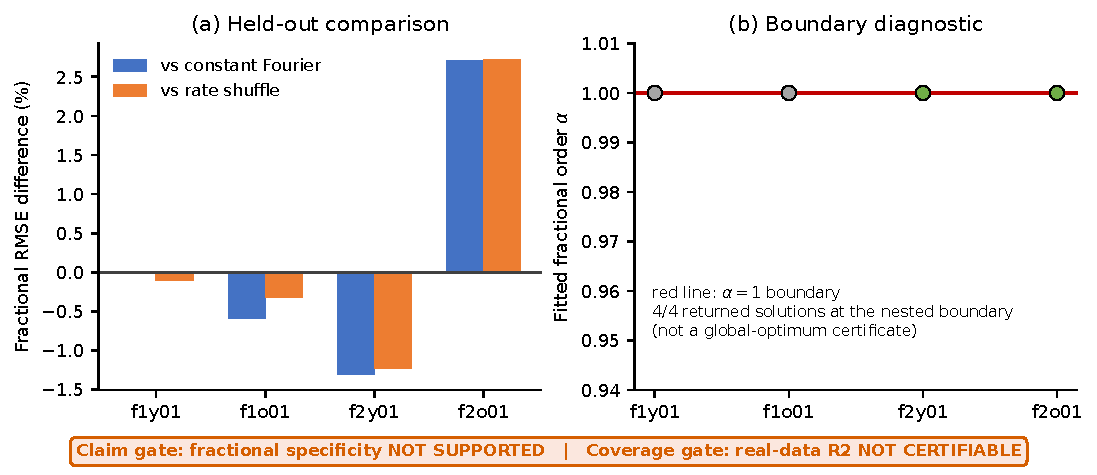
\includegraphics[width=0.97\linewidth]{figures/fantasia_pilot_summary.pdf}
\caption{Design-locked Fantasia engineering pilot.  Every fitted free order
lands at the admissible boundary $\alpha=1$.  A negative RMSE percentage
difference favors the fractional fit; the two locked records disagree in
direction against the constant and rate-shuffle controls.  The figure is
descriptive and does not represent a certified R2 inference.}
\label{fig:fantasia-main}
\end{figure}

The material-improvement threshold was fixed at 0.1\% relative RMSE.  All
four returned free-order fits terminated at $\alpha=1$, and the
fractional/nested RMSE
ratio was numerically one in 4/4 records.  Thus the fractional model had zero
material wins over its $\alpha=1$ submodel.  On locked f2y01 it improved on the
constant and shuffle controls by about 1.30\% and 1.23\%, whereas on locked
f2o01 it was worse by about 2.71\% and 2.72\%.  The directions disagree.
The identification/validation heart-rate ranges (Hz) were respectively
1.105--1.421/1.048--1.581 (f1y01),
0.941--1.100/0.911--1.219 (f1o01),
1.085--1.292/1.030--1.475 (f2y01), and
1.038--1.351/0.927--1.152 (f2o01).  The returned fractional-model
$\lambda$ values were 32.812, 0.001, 2.0045, and 0.001; the f1o01 and f2o01
solutions hit the predeclared lower bound.  These boundary hits and the
uncontrolled, substantially overlapping rate ranges further limit
interpretation.
Accordingly,
\[
 \text{distinct fractional-order evidence}=\status{NOT\_SUPPORTED},
\]
and confirmatory rate-response evidence is also
\status{NOT\_SUPPORTED}.

All four real records remain \status{NOT\_CERTIFIABLE}.  Missing primitives
include annotation-timing and whole-window phase-warp error,
measurement-noise and model-discrepancy envelopes, finite-dwell and prehistory
bounds, sampling/quadrature and subsampling anti-alias bounds, omitted-harmonic
tail/leakage, ADC-gain and analog-front-end calibration uncertainty, and a
complete interval enclosure of $G$ and the right-hand-side accumulation.
Empirical validation residuals are not used to fill these bounds.

\section{Discussion}

\subsection{What the theory establishes}

The global quotient theorem provides a clean answer to the structural
question posed in the introduction.  Positive real damping adds a phase
constraint that makes two complete complex rate responses sufficient despite
the unknown complex morphology.  This is stronger than counting complex
equations, because it identifies the complete nuisance quotient and its
physical image.  The multi-rate result then separates estimation from model
checking: two rates are exactly determined; a third rate creates redundancy.

The result is useful only when the common-gauge protocol is credible.
Theorems~\ref{thm:drift-main} and Proposition~\ref{prop:gauge-no-go-main} show
why morphology handling cannot be an informal preprocessing choice.  Allowing
arbitrary complex changes removes all order information, and even a small
positive independent disk prevents a singleton conclusion in the stated
two-rate problem.  These are not merely numerical conditioning warnings; they
are identifiability limits.

The finite-record layer gives a second separation.  WLS geometry converts a
valid residual envelope to a coefficient disk, but cannot create that
envelope.  Hardware, annotations, front-end response, memory tails, and model
discrepancy need independent evidence.  Fail-closed replay protects this
boundary against accidentally reusing a fitted residual as both estimate and
coverage proof.

\subsection{Interpretation of the negative pilot}

The Fantasia result does not refute every fractional ECG model.  It says that,
under this frozen scalar harmonic family and four-record engineering design,
the additional order freedom did not separate from the $\alpha=1$ boundary.
Nor did the two locked records show a consistent advantage over simpler
controls.  This is precisely the kind of result that a nested baseline and
negative control should reveal before a larger study.

The useful positive outcome is narrower: fixed-phase segmentation, two-sided
joint complex WLS, source/payload hashing, deterministic replay, temporal
guarding, and model-comparison code all operated on long external ECG records.
Those engineering checks justify a future controlled multi-rate acquisition;
they do not justify a physiological-order claim.

\subsection{Limitations and next experiments}

First, the scalar steady harmonic surrogate omits multichannel propagation,
beat morphology dynamics, autonomic covariates, and spatial cardiac states.
Its order should not be interpreted as tissue-level memory.  Second, the
finite-frequency rational-interpolation result prevents mechanism attribution
from harmonic agreement alone.  Held-out transients and integer-order
rational baselines are necessary.

Third, the current real-data evidence closes WLS execution replay but not R2
coverage.  The missing primitive bounds listed above must be obtained through
instrument calibration, controlled annotation studies, interval
reconstruction, and an independently specified model-discrepancy contract.
Fourth, the four records are too few for population inference and only two
were locked engineering-validation records.  No age-group conclusion is
drawn.  Fifth, the observed heart-rate range was not optimized using
Theorem~\ref{thm:design-main}; uncontrolled resting data can be structurally
valid yet practically uninformative.

A decisive follow-up should therefore use controlled, sufficiently separated
rate plateaus; one fixed acquisition chain; explicit dwell and prehistory
control; calibration data disjoint from subject-specific identification and
future validation; and a predeclared R2 budget.  The experiment should proceed
only if the optimized separation modulus exceeds two at the target order
resolution.  A larger ECG cohort or learned centre estimator is secondary:
neither can replace missing coverage primitives.

\section{Conclusion}

We have presented a control-theoretic identifiability and certification
framework for a fractional surface-ECG harmonic surrogate.  The core theorem
shows that two exact complex rate responses uniquely recover order and damping
modulo a common complex morphology/lead gauge, while one response is
insufficient.  Joint response disks, independently calibrated finite-record
bounds, validated Gram margins, and fail-closed replay extend the structural
result toward auditable data analysis.  The accompanying no-go and minimax
results define when the problem cannot deliver a narrow order set and how a
future rate-window experiment should be designed.

The reported real-data pilot is intentionally retained as a negative result: all
four fitted orders equal one, the nested integer-order model is not improved,
and the necessary real-data error bounds are incomplete.  The current
conclusions are therefore \status{NOT\_SUPPORTED} for distinct fractional
order and \status{NOT\_CERTIFIABLE} for real-ECG set inference.  Preserving
those conclusions is essential to the credibility of any later, larger
validation.

\section*{Reproducibility and evidence availability}

The repository contains the theory-core supplement, protocol template,
source-code certificate issuers/replayers, deterministic test scripts, the
sealed exact-sample and two-rate summaries, and the derived Fantasia evidence
bundle.  Raw ECG records remain outside the repository; all 12 selected files
match the official Fantasia v1.0.0 SHA-256 manifest.  The Fantasia bundle
contains only manifests, derived coefficients, execution records (including
derived beat indices), comparisons, and checksums under the source-dataset
attribution boundary.  Production-source hashes, package/runtime identifiers,
and reproduction commands are recorded with the evidence objects.  The main
manuscript does not treat generated point estimates as certified disks.

\begin{thebibliography}{99}
\small

\bibitem{mcsharry2003}
P. E. McSharry, G. D. Clifford, L. Tarassenko, and L. A. Smith,
``A dynamical model for generating synthetic electrocardiogram signals,''
\emph{IEEE Transactions on Biomedical Engineering}, vol. 50, no. 3,
pp. 289--294, 2003.
\href{https://doi.org/10.1109/TBME.2003.808805}{doi:10.1109/TBME.2003.808805}.

\bibitem{sameni2007}
R. Sameni, M. B. Shamsollahi, C. Jutten, and G. D. Clifford,
``A nonlinear Bayesian filtering framework for ECG denoising,''
\emph{IEEE Transactions on Biomedical Engineering}, vol. 54, no. 12,
pp. 2172--2185, 2007.
\href{https://doi.org/10.1109/TBME.2007.897817}{doi:10.1109/TBME.2007.897817}.

\bibitem{sierociuk2006}
D. Sierociuk and A. Dzieli\'nski,
``Fractional Kalman filter algorithm for the states, parameters and order of
fractional system estimation,''
\emph{International Journal of Applied Mathematics and Computer Science},
vol. 16, no. 1, pp. 129--140, 2006.

\bibitem{sierociuk2021}
D. Sierociuk and M. Macias,
``Triple estimation of fractional variable order, parameters, and state
variables based on the unscented fractional order Kalman filter,''
\emph{Sensors}, vol. 21, no. 23, 8159, 2021.
\href{https://doi.org/10.3390/s21238159}{doi:10.3390/s21238159}.

\bibitem{yu2026}
W. Yu, Y. Zhang, R. Chen, W. Zhu, C. Wen, and Y. Chen,
``A fractional high-order extended Kalman filter for fractional-order
nonlinear systems,'' \emph{ISA Transactions}, vol. 171, pp. 152--162, 2026.
\href{https://doi.org/10.1016/j.isatra.2026.02.020}{doi:10.1016/j.isatra.2026.02.020}.

\bibitem{nazarian2010}
N. Nazarian, M. Haeri, and M. S. Tavazoei,
``Identifiability of fractional order systems using input output frequency
contents,'' \emph{ISA Transactions}, vol. 49, pp. 207--214, 2010.
\href{https://doi.org/10.1016/j.isatra.2009.11.007}{doi:10.1016/j.isatra.2009.11.007}.

\bibitem{tavazoei2009}
M. S. Tavazoei and M. Haeri,
``A proof for non existence of periodic solutions in time invariant
fractional order systems,'' \emph{Automatica}, vol. 45, no. 8,
pp. 1886--1890, 2009.
\href{https://doi.org/10.1016/j.automatica.2009.04.001}{doi:10.1016/j.automatica.2009.04.001}.

\bibitem{duan2022}
J.-S. Duan, Y.-J. Lan, and M. Li,
``A comparative study of responses of fractional oscillator to sinusoidal
excitation in the Weyl and Caputo senses,'' \emph{Fractal and Fractional},
vol. 6, no. 12, art. 692, 2022.
\href{https://doi.org/10.3390/fractalfract6120692}{doi:10.3390/fractalfract6120692}.

\bibitem{malti2010}
R. Malti, T. Ra\"{\i}ssi, M. Thomassin, and F. Khemane,
``Set membership parameter estimation of fractional models based on bounded
frequency domain data,'' \emph{Communications in Nonlinear Science and
Numerical Simulation}, vol. 15, pp. 927--938, 2010.
\href{https://doi.org/10.1016/j.cnsns.2009.05.005}{doi:10.1016/j.cnsns.2009.05.005}.

\bibitem{khemane2012}
F. Khemane, R. Malti, T. Raissi, and X. Moreau,
``Robust estimation of fractional models in the frequency domain using set
membership methods,'' \emph{Signal Processing}, vol. 92, pp. 1591--1601,
2012.
\href{https://doi.org/10.1016/j.sigpro.2011.12.008}{doi:10.1016/j.sigpro.2011.12.008}.

\bibitem{abrashov2017}
S. Abrashov, R. Malti, M. Moze, X. Moreau, F. Aioun, and F. Guillemard,
``Simple and robust experiment design for system identification using
fractional models,'' \emph{IEEE Transactions on Automatic Control}, vol. 62,
pp. 2648--2658, 2017.
\href{https://doi.org/10.1109/TAC.2016.2614910}{doi:10.1109/TAC.2016.2614910}.

\bibitem{karimshoushtari2020}
M. Karimshoushtari and C. Novara,
``Design of experiments for nonlinear system identification: A set membership
approach,'' \emph{Automatica}, vol. 119, 109036, 2020.
\href{https://doi.org/10.1016/j.automatica.2020.109036}{doi:10.1016/j.automatica.2020.109036}.

\bibitem{das2013}
S. Das and K. Maharatna,
``Fractional dynamical model for the generation of ECG like signals from
filtered coupled Van-der-Pol oscillators,''
\emph{Computer Methods and Programs in Biomedicine}, vol. 112, no. 3,
pp. 490--507, 2013.
\href{https://doi.org/10.1016/j.cmpb.2013.08.012}{doi:10.1016/j.cmpb.2013.08.012}.

\bibitem{templos2021}
D. J. Templos-Hernandez et al.,
``A fractional-order approach to cardiac rhythm analysis,''
\emph{Chaos, Solitons \& Fractals}, vol. 145, 110942, 2021.
\href{https://doi.org/10.1016/j.chaos.2021.110942}{doi:10.1016/j.chaos.2021.110942}.

\bibitem{takha2024}
A. Takha, M. L. Talbi, and P. Ravier,
``Fractional calculus integration for improved ECG modeling: A McSharry model
expansion,'' \emph{Medical Engineering \& Physics}, vol. 132, 104237, 2024.
\href{https://doi.org/10.1016/j.medengphy.2024.104237}{doi:10.1016/j.medengphy.2024.104237}.

\bibitem{gillette2021}
K. Gillette et al.,
``A framework for the generation of digital twins of cardiac
electrophysiology from clinical 12-leads ECGs,''
\emph{Medical Image Analysis}, vol. 71, 102080, 2021.
\href{https://doi.org/10.1016/j.media.2021.102080}{doi:10.1016/j.media.2021.102080}.

\bibitem{grandits2025}
T. Grandits, K. Gillette, G. Plank, and S. Pezzuto,
``Accurate and efficient cardiac digital twin from surface ECGs: Insights
into identifiability of ventricular conduction system,''
\emph{Medical Image Analysis}, vol. 105, 103641, 2025.
\href{https://doi.org/10.1016/j.media.2025.103641}{doi:10.1016/j.media.2025.103641}.

\bibitem{rauhmalti2023}
A. Rauh and R. Malti,
``Quantification of time-domain truncation errors for the reinitialization of
fractional integrators,'' \emph{Acta Cybernetica}, vol. 26, pp. 105--128,
2023.
\href{https://doi.org/10.14232/actacyb.296010}{doi:10.14232/actacyb.296010}.

\bibitem{rauhlahme2025}
A. Rauh and M. Lahme,
``Observer-based error correction in finite memory approaches for pseudo
state estimation of fractional dynamic models,''
\emph{Annual Reviews in Control}, vol. 60, 101018, 2025.
\href{https://doi.org/10.1016/j.arcontrol.2025.101018}{doi:10.1016/j.arcontrol.2025.101018}.

\bibitem{neumaier1989}
A. Neumaier,
``Rigorous sensitivity analysis for parameter-dependent systems of
equations,'' \emph{Journal of Mathematical Analysis and Applications},
vol. 144, pp. 16--25, 1989.
\href{https://doi.org/10.1016/0022-247X(89)90357-0}{doi:10.1016/0022-247X(89)90357-0}.

\bibitem{rump2010}
S. M. Rump,
``Verification methods: Rigorous results using floating-point arithmetic,''
\emph{Acta Numerica}, vol. 19, pp. 287--449, 2010.
\href{https://doi.org/10.1017/S096249291000005X}{doi:10.1017/S096249291000005X}.

\bibitem{goldsztejn2006}
A. Goldsztejn and L. Jaulin,
``Inner and outer approximations of existentially quantified equality
constraints,'' in \emph{CP 2006}, LNCS 4204, pp. 198--212, 2006.
\href{https://doi.org/10.1007/11889205_16}{doi:10.1007/11889205\_16}.

\bibitem{ponleitner2021}
B. Ponleitner and H. Schichl,
``Exclusion regions for parameter-dependent systems of equations,''
\emph{Journal of Global Optimization}, vol. 81, pp. 621--644, 2021.
\href{https://doi.org/10.1007/s10898-021-01082-3}{doi:10.1007/s10898-021-01082-3}.

\bibitem{pollard1948}
H. Pollard,
``The completely monotonic character of the Mittag--Leffler function
$E_\alpha(-x)$,'' \emph{Bulletin of the American Mathematical Society},
vol. 54, pp. 1115--1116, 1948.
\href{https://doi.org/10.1090/S0002-9904-1948-09132-7}{doi:10.1090/S0002-9904-1948-09132-7}.

\bibitem{simon2014}
T. Simon,
``Comparing Fr\'echet and positive stable laws,''
\emph{Electronic Journal of Probability}, vol. 19, paper 16, pp. 1--25,
2014.
\href{https://doi.org/10.1214/EJP.v19-3058}{doi:10.1214/EJP.v19-3058}.

\bibitem{iyengar1996}
N. Iyengar, C.-K. Peng, R. Morin, A. L. Goldberger, and L. A. Lipsitz,
``Age-related alterations in the fractal scaling of cardiac interbeat
interval dynamics,'' \emph{American Journal of Physiology--Regulatory,
Integrative and Comparative Physiology}, vol. 271, no. 4,
pp. R1078--R1084, 1996.
\href{https://doi.org/10.1152/ajpregu.1996.271.4.R1078}{doi:10.1152/ajpregu.1996.271.4.R1078}.

\bibitem{fantasia2003}
C.-K. Peng and L. Lipsitz,
``Fantasia Database,'' PhysioNet, version 1.0.0, 2003.
\href{https://doi.org/10.13026/C2RG61}{doi:10.13026/C2RG61}.

\bibitem{goldberger2000}
A. L. Goldberger, L. A. N. Amaral, L. Glass, J. M. Hausdorff,
P. Ch. Ivanov, R. G. Mark, J. E. Mietus, G. B. Moody, C.-K. Peng, and
H. E. Stanley,
``PhysioBank, PhysioToolkit, and PhysioNet: Components of a new research
resource for complex physiologic signals,'' \emph{Circulation}, vol. 101,
no. 23, pp. e215--e220, 2000.
\href{https://doi.org/10.1161/01.CIR.101.23.e215}{doi:10.1161/01.CIR.101.23.e215}.

\bibitem{johansson2017}
F. Johansson,
``Arb: Efficient arbitrary-precision midpoint-radius interval arithmetic,''
\emph{IEEE Transactions on Computers}, vol. 66, no. 8,
pp. 1281--1292, 2017.
\href{https://doi.org/10.1109/TC.2017.2690633}{doi:10.1109/TC.2017.2690633}.

\end{thebibliography}

\end{document}
